% =========================================================
\subsubsection{Isometries}
\label{sec:isometries}
% =========================================================

% ---- Toolkit ----
\begin{tcolorbox}[colback=gray!6, colframe=gray!40, arc=2pt,
  left=6pt, right=6pt, top=4pt, bottom=4pt,
  title={\small\textbf{Isometries --- Quick Reference}},
  fonttitle=\small\bfseries]
\small
\begin{tabular}{l l l l}
\toprule
\textbf{Label} & \textbf{Statement} & \textbf{Proof method} & \textbf{Detail} \\
\midrule
D\ref{def:isometry}
  & $d_Y(f(x),f(y)) = d_X(x,y)$; bijective case = isometric isomorphism
  & Definition
  & \hyperref[def:isometry]{$\downarrow$} \\
D\ref{def:subspace-metric}
  & $(A, d|_A)$ is a metric space for any $A \subseteq X$
  & Definition
  & \hyperref[def:subspace-metric]{$\downarrow$} \\
P\ref{prop:isometry-injective}
  & Every isometry is injective
  & $d_X(x,y)=0 \Rightarrow x=y$
  & \hyperref[prop:isometry-injective]{$\downarrow$} \\
P\ref{prop:inverse-isometry}
  & $f$ bijective isometry $\Rightarrow$ $f^{-1}$ is an isometry
  & Direct from definition
  & \hyperref[prop:inverse-isometry]{$\downarrow$} \\
P\ref{prop:isometry-preserves-balls}
  & $f(B_r(x)) = B_r(f(x))$
  & Direct from definition
  & \hyperref[prop:isometry-preserves-balls]{$\downarrow$} \\
P\ref{prop:isometry-preserves-diameter}
  & $\operatorname{diam}(f(A)) = \operatorname{diam}(A)$
  & Direct from definition
  & \hyperref[prop:isometry-preserves-diameter]{$\downarrow$} \\
P\ref{prop:isometry-preserves-open}
  & Bijective isometry preserves open and closed sets
  & Via ball preservation
  & \hyperref[prop:isometry-preserves-open]{$\downarrow$} \\
P\ref{prop:isometry-preserves-convergence}
  & Bijective isometry preserves convergence and Cauchy sequences
  & Direct from definition
  & \hyperref[prop:isometry-preserves-convergence]{$\downarrow$} \\
P\ref{prop:isometry-group}
  & $\mathrm{Isom}(X,d)$ is a group under composition
  & Group axiom verification
  & \hyperref[prop:isometry-group]{$\downarrow$} \\
D\ref{def:rigid-motion}
  & Rigid motion = bijective isometry $\mathbb{R}^n \to \mathbb{R}^n$
  & Definition
  & \hyperref[def:rigid-motion]{$\downarrow$} \\
T\ref{thm:classification-rigid-motions}
  & Every rigid motion = orthogonal map $+$ translation
  & Structure theorem
  & \hyperref[thm:classification-rigid-motions]{$\downarrow$} \\
\bottomrule
\end{tabular}
\end{tcolorbox}

% ---- Isometry and Isometric Isomorphism ----
\begin{tcolorbox}[colback=propbox, colframe=propborder, arc=2pt,
  left=6pt, right=6pt, top=4pt, bottom=4pt,
  title={\small\textbf{Definition (Isometry; Isometric Isomorphism)}},
  fonttitle=\small\bfseries]
\begin{definition}[Isometry; Isometric Isomorphism]
\label{def:isometry}
Let $(X,d_X)$ and $(Y,d_Y)$ be metric spaces.
A map $f : X \to Y$ is called an \emph{isometry} if
\[
d_Y\bigl(f(x),\, f(y)\bigr) = d_X(x,y)
\quad \forall\, x,y \in X.
\]
A bijective isometry is called an \emph{isometric isomorphism}.
If such a map exists, $(X,d_X)$ and $(Y,d_Y)$ are said to be
\emph{isometric}, written $X \cong Y$.
\end{definition}
\end{tcolorbox}

\begin{remark*}[Fully quantified form]
\[
f\ \text{is an isometry}
\iff
\forall x, y \in X,\quad
d_Y(f(x), f(y)) = d_X(x,y).
\]
\end{remark*}

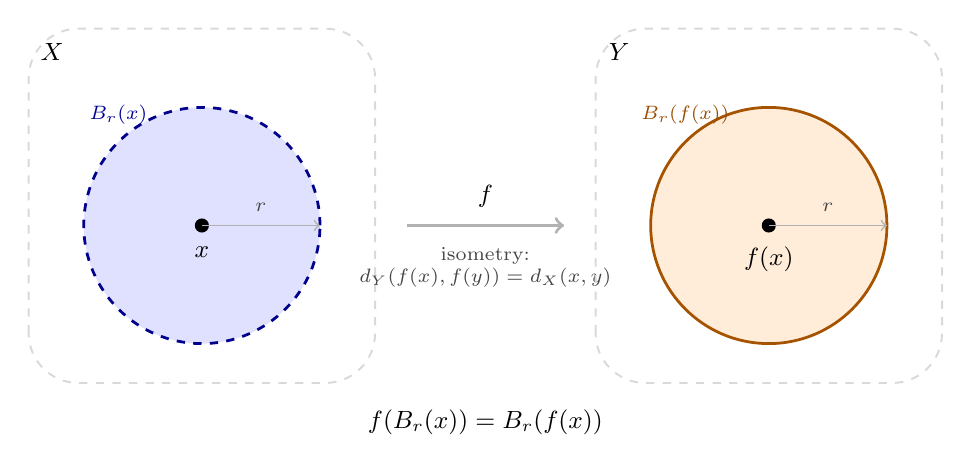
\begin{tikzpicture}[
  dot/.style={circle,fill,inner sep=1.8pt},
  lbl/.style={font=\small},
  sublbl/.style={font=\scriptsize,text=gray!55!black}
]

% ---- LEFT: space X ----
\begin{scope}[shift={(-3.6,0)}]
  % Background blob for X
  \draw[gray!30, line width=0.7pt, dashed, rounded corners=18pt]
    (-2.2,-2.0) rectangle (2.2,2.5);
  \node[lbl,font=\small\itshape] at (-1.9,2.2) {$X$};

  % Ball B_r(x)
  \fill[blue!12] (0,0) circle (1.5cm);
  \draw[blue!55!black, dashed, line width=1.0pt] (0,0) circle (1.5cm);

  % Centre x
  \node[dot,fill=black] at (0,0) {};
  \node[lbl,anchor=north] at (0,-0.15) {$x$};

  % Radius arrow
  \draw[gray!60,->,line width=0.6pt] (0,0) -- (1.5,0);
  \node[sublbl,anchor=south] at (0.75,0.05) {$r$};

  % Label
  \node[sublbl,text=blue!60!black,anchor=south]
    at ({-1.5*0.707},{1.5*0.707+0.1}) {$B_r(x)$};
\end{scope}

% ---- Arrow f in middle ----
\draw[->,line width=1.2pt,gray!60] (-1.0,0) -- (1.0,0);
\node[lbl,anchor=south] at (0,0.1) {$f$};
\node[sublbl,anchor=north,align=center] at (0,-0.15)
  {isometry:\\$d_Y(f(x),f(y))=d_X(x,y)$};

% ---- RIGHT: space Y ----
\begin{scope}[shift={(3.6,0)}]
  \draw[gray!30, line width=0.7pt, dashed, rounded corners=18pt]
    (-2.2,-2.0) rectangle (2.2,2.5);
  \node[lbl,font=\small\itshape] at (-1.9,2.2) {$Y$};

  % Ball B_r(f(x)) — same radius
  \fill[orange!15] (0,0) circle (1.5cm);
  \draw[orange!65!black, line width=1.0pt] (0,0) circle (1.5cm);

  % Centre f(x)
  \node[dot,fill=black] at (0,0) {};
  \node[lbl,anchor=north] at (0,-0.15) {$f(x)$};

  % Radius arrow
  \draw[gray!60,->,line width=0.6pt] (0,0) -- (1.5,0);
  \node[sublbl,anchor=south] at (0.75,0.05) {$r$};

  % Label
  \node[sublbl,text=orange!60!black,anchor=south]
    at ({-1.5*0.707},{1.5*0.707+0.1}) {$B_r(f(x))$};
\end{scope}

% Footer
\node[lbl,align=center] at (0,-2.5)
  {$f(B_r(x)) = B_r(f(x))$};
\end{tikzpicture}

\begin{remark*}[Intuition]
An isometry is a distance-preserving map: the geometry of $(X,d_X)$
is reproduced exactly in $(Y,d_Y)$ by $f$.
An isometric isomorphism is stronger --- it is a distance-preserving
bijection, meaning $(X,d_X)$ and $(Y,d_Y)$ are the same metric space
up to relabelling of points.
\end{remark*}

\begin{remark*}[Relation to topology]
An isometry is automatically a homeomorphism onto its image (a topological
embedding), and a bijective isometry is a homeomorphism.
Isometries are to metric spaces what isomorphisms are to algebraic structures:
they are the structure-preserving maps.
\end{remark*}

% ---- Subspace metric ----
\begin{tcolorbox}[colback=propbox, colframe=propborder, arc=2pt,
  left=6pt, right=6pt, top=4pt, bottom=4pt,
  title={\small\textbf{Definition (Subspace Metric)}},
  fonttitle=\small\bfseries]
\begin{definition}[Subspace Metric]
\label{def:subspace-metric}
Let $(X,d)$ be a metric space and $A \subseteq X$.
The \emph{subspace metric} on $A$ is the restriction
\[
d|_A : A \times A \to \mathbb{R},
\qquad
d|_A(x,y) := d(x,y).
\]
The pair $(A, d|_A)$ is called a \emph{metric subspace} of $(X,d)$.
\end{definition}
\end{tcolorbox}

\begin{remark*}[The inclusion map is an isometry]
The inclusion $\iota : (A, d|_A) \hookrightarrow (X,d)$, $\iota(x) = x$,
satisfies $d(\iota(x), \iota(y)) = d(x,y) = d|_A(x,y)$ for all $x,y \in A$.
So $\iota$ is an isometry.
This makes the subspace metric the canonical example of an isometry:
every subset is isometrically embedded in its ambient space.
\end{remark*}

\begin{remark*}[Openness in subspace vs.\ ambient space]
A set $U \subseteq A$ is open in $(A, d|_A)$ if and only if
$U = A \cap V$ for some open $V \subseteq X$.
Openness in $A$ and openness in $X$ can therefore differ:
$[0, \tfrac{1}{2})$ is open in $[0,1]$ under the subspace metric
(it equals $B_{1/2}(0) \cap [0,1]$) but is not open in $\mathbb{R}$.
\end{remark*}

% ---- Fundamental Properties ----

\begin{proposition}[\texorpdfstring{%
  \hyperref[prf:isometry-injective]{Injectivity of Isometries}%
}{Injectivity of Isometries}]
\label{prop:isometry-injective}
Every isometry $f : X \to Y$ is injective.
\end{proposition}

\begin{remark*}[Proof shape]
If $f(x) = f(y)$ then $d_X(x,y) = d_Y(f(x),f(y)) = d_Y(f(x),f(x)) = 0$,
so $x = y$ by the identity axiom of $d_X$.
\end{remark*}

\begin{proposition}[\texorpdfstring{%
  \hyperref[prf:inverse-isometry]{Inverse of a Bijective Isometry}%
}{Inverse of a Bijective Isometry}]
\label{prop:inverse-isometry}
If $f : X \to Y$ is a bijective isometry then $f^{-1} : Y \to X$
is also a bijective isometry.
\end{proposition}

\begin{remark*}[Consequence]
This shows that being isometric is a symmetric relation: if $X \cong Y$
then $Y \cong X$.
Combined with composition (below), it makes isometry an equivalence
relation on metric spaces.
\end{remark*}

\begin{proposition}[\texorpdfstring{%
  \hyperref[prf:isometry-preserves-balls]{Preservation of Open Balls}%
}{Preservation of Open Balls}]
\label{prop:isometry-preserves-balls}
If $f : X \to Y$ is an isometry then for all $x \in X$ and $r > 0$,
\[
f\!\left(B_r(x)\right) = B_r\!\left(f(x)\right).
\]
\end{proposition}

\begin{remark*}[Intuition]
An isometry maps balls to balls of the same radius centred at the image
of the centre.
This is the metric-geometric content of distance preservation.
\end{remark*}

\begin{proposition}[\texorpdfstring{%
  \hyperref[prf:isometry-preserves-diameter]{Preservation of Diameter}%
}{Preservation of Diameter}]
\label{prop:isometry-preserves-diameter}
If $f : X \to Y$ is an isometry then for every $A \subseteq X$,
\[
\operatorname{diam}(f(A)) = \operatorname{diam}(A).
\]
\end{proposition}

\begin{proposition}[\texorpdfstring{%
  \hyperref[prf:isometry-preserves-open]{Preservation of Open and Closed Sets}%
}{Preservation of Open and Closed Sets}]
\label{prop:isometry-preserves-open}
If $f : X \to Y$ is a bijective isometry then $U \subseteq X$ is open
(respectively closed) if and only if $f(U) \subseteq Y$ is open
(respectively closed).
\end{proposition}

\begin{remark*}[Consequence]
A bijective isometry is a homeomorphism.
Equivalently, the topology induced by $d_X$ and the topology induced
by $d_Y$ are in bijective correspondence via $f$.
\end{remark*}

\begin{proposition}[\texorpdfstring{%
  \hyperref[prf:isometry-preserves-convergence]{Preservation of Convergence and Cauchy Sequences}%
}{Preservation of Convergence and Cauchy Sequences}]
\label{prop:isometry-preserves-convergence}
If $f : X \to Y$ is a bijective isometry then:
\begin{enumerate}[label=(\roman*)]
  \item $(x_n)$ converges in $X$ if and only if $(f(x_n))$ converges in $Y$,
        with $x_n \to x \iff f(x_n) \to f(x)$.
  \item $(x_n)$ is Cauchy in $X$ if and only if $(f(x_n))$ is Cauchy in $Y$.
  \item $X$ is complete if and only if $Y$ is complete.
  \item $X$ is compact if and only if $Y$ is compact.
\end{enumerate}
\end{proposition}

\begin{remark*}[Consequence]
Completeness and compactness are metric invariants: they depend on the
distances, not on the underlying set.
In particular, isometric metric spaces are interchangeable for all
purposes of analysis.
\end{remark*}


\begin{proposition}[\texorpdfstring{%
  \hyperref[prf:isometry-preserves-bounded]{Preservation of Boundedness}%
}{Preservation of Boundedness}]
\label{prop:isometry-preserves-bounded}
If $f : X \to Y$ is an isometry and $A \subseteq X$, then $A$ is bounded
if and only if $f(A)$ is bounded.
\end{proposition}

\begin{remark*}[Proof shape]
Recall that a set $A \subseteq X$ is bounded if
\[
\operatorname{diam}(A) < \infty.
\]

By Proposition~\ref{prop:isometry-preserves-diameter},
\[
\operatorname{diam}(f(A)) = \operatorname{diam}(A).
\]

Thus $\operatorname{diam}(A)$ is finite if and only if
$\operatorname{diam}(f(A))$ is finite, so $A$ is bounded
if and only if $f(A)$ is bounded.
\end{remark*}


% ---- Isometry group ----

\begin{proposition}[\texorpdfstring{%
  \hyperref[prf:isometry-group]{Isometry Group}%
}{Isometry Group}]
\label{prop:isometry-group}
Let $(X,d)$ be a metric space.
The set
\[
\mathrm{Isom}(X,d)
:= \{\, f : X \to X \mid f\ \text{is a bijective isometry}\,\}
\]
is a group under composition.
\end{proposition}

\begin{remark*}[Intuition]
The isometry group captures all the symmetries of the metric space.
For $\mathbb{R}^n$ with the Euclidean metric this is the full Euclidean
group $\mathrm{E}(n)$, generated by rotations, reflections, and translations.
For a discrete metric space on $n$ points it is the symmetric group $S_n$.
\end{remark*}

% =========================================================
\subsubsection{Rigid Motions in Euclidean Space}
\label{sec:rigid-motions}
% =========================================================

\begin{tcolorbox}[colback=propbox, colframe=propborder, arc=2pt,
  left=6pt, right=6pt, top=4pt, bottom=4pt,
  title={\small\textbf{Definition (Rigid Motion)}},
  fonttitle=\small\bfseries]
\begin{definition}[Rigid Motion]
\label{def:rigid-motion}
A \emph{rigid motion} of $\mathbb{R}^n$ is a bijective isometry
$f : \mathbb{R}^n \to \mathbb{R}^n$
with respect to the Euclidean metric $\|\cdot\|_2$.
\end{definition}
\end{tcolorbox}

\begin{tikzpicture}[
  dot/.style={circle,fill,inner sep=1.4pt},
  lbl/.style={font=\small},
  sublbl/.style={font=\scriptsize,text=gray!55!black}
]

% Base triangle vertices (used in all panels)
% A=(0,0), B=(1.4,0), C=(0.5,1.1)
\def\drawTriangle#1#2#3#4{  % Ax Ay Bx By Cx Cy + fill colour
}

% ---- Panel 1: Original ----
\begin{scope}[shift={(0,0)}]
  \coordinate (A) at (0,0);
  \coordinate (B) at (1.4,0);
  \coordinate (C) at (0.5,1.1);
  \fill[blue!20] (A)--(B)--(C)--cycle;
  \draw[blue!65!black,line width=1.1pt] (A)--(B)--(C)--cycle;
  \node[dot,fill=blue!70!black] at (A) {};
  \node[dot,fill=blue!70!black] at (B) {};
  \node[dot,fill=blue!70!black] at (C) {};
  \node[sublbl,anchor=north] at ($(A)+(0,-0.15)$) {$A$};
  \node[sublbl,anchor=north] at ($(B)+(0,-0.15)$) {$B$};
  \node[sublbl,anchor=south] at ($(C)+(0,0.12)$)  {$C$};
  \node[lbl,font=\small\bfseries,anchor=north] at (0.7,-0.55) {Original};
\end{scope}

% ---- Panel 2: Rotation 45° ----
\begin{scope}[shift={(3.2,0)}]
  % Rotate 45°: (x,y) -> (x cos45 - y sin45, x sin45 + y cos45)
  \pgfmathsetmacro{\cs}{cos(45)}
  \pgfmathsetmacro{\sn}{sin(45)}
  \coordinate (A) at (0,0);
  \coordinate (B) at ({1.4*\cs},{1.4*\sn});
  \coordinate (C) at ({0.5*\cs-1.1*\sn},{0.5*\sn+1.1*\cs});
  \fill[green!15!blue!15] (A)--(B)--(C)--cycle;
  \draw[green!50!blue!70,line width=1.1pt] (A)--(B)--(C)--cycle;
  \node[dot,fill=green!50!blue!70] at (A) {};
  \node[dot,fill=green!50!blue!70] at (B) {};
  \node[dot,fill=green!50!blue!70] at (C) {};
  % Rotation arc indicator
  \draw[gray!55,->,line width=0.7pt] (0.9,0) arc(0:45:0.9);
  \node[sublbl,anchor=west] at (0.95,0.45) {$45°$};
  \node[lbl,font=\small\bfseries,anchor=north] at (0.5,-0.55) {Rotation};
\end{scope}

% ---- Panel 3: Translation ----
\begin{scope}[shift={(6.1,0)}]
  % Original (ghost)
  \draw[blue!25,line width=0.7pt,dashed] (0,0)--(1.4,0)--(0.5,1.1)--cycle;
  % Translated by (0.6,0.5)
  \coordinate (A) at (0.6,0.5);
  \coordinate (B) at (2.0,0.5);
  \coordinate (C) at (1.1,1.6);
  \fill[orange!20] (A)--(B)--(C)--cycle;
  \draw[orange!70!black,line width=1.1pt] (A)--(B)--(C)--cycle;
  \node[dot,fill=orange!70!black] at (A) {};
  \node[dot,fill=orange!70!black] at (B) {};
  \node[dot,fill=orange!70!black] at (C) {};
  % Translation arrow
  \draw[gray!55,->,line width=0.7pt] (0.1,0.1) -- (0.48,0.4);
  \node[sublbl,anchor=east] at (0.1,0.25) {$+a$};
  \node[lbl,font=\small\bfseries,anchor=north] at (1.0,-0.55) {Translation};
\end{scope}

% ---- Panel 4: Reflection across vertical axis ----
\begin{scope}[shift={(9.2,0)}]
  % Reflection: x -> -x+1.4 (flip around x=0.7)
  \coordinate (A) at (1.4,0);
  \coordinate (B) at (0.0,0);
  \coordinate (C) at (0.9,1.1);
  \fill[red!12] (A)--(B)--(C)--cycle;
  \draw[red!60!black,line width=1.1pt] (A)--(B)--(C)--cycle;
  \node[dot,fill=red!60!black] at (A) {};
  \node[dot,fill=red!60!black] at (B) {};
  \node[dot,fill=red!60!black] at (C) {};
  % Mirror line
  \draw[gray!45,line width=0.7pt,dashed] (0.7,-0.4) -- (0.7,1.5);
  \node[sublbl,text=gray!50,anchor=south] at (0.7,1.52) {axis};
  \node[lbl,font=\small\bfseries,anchor=north] at (0.7,-0.55) {Reflection};
\end{scope}

\end{tikzpicture}

\begin{remark*}[Intuition]
A rigid motion moves points in $\mathbb{R}^n$ without stretching,
compressing, or shearing: all pairwise distances are preserved.
The term ``rigid'' reflects that such a motion cannot deform the shape
of any figure.
\end{remark*}

\begin{proposition}[\texorpdfstring{%
  \hyperref[prf:rotations-are-isometries]{Rotations are Isometries}%
}{Rotations are Isometries}]
\label{prop:rotations-are-isometries}
Let $R : \mathbb{R}^n \to \mathbb{R}^n$ be an orthogonal linear map
(i.e.\ $R^\top R = I$). Then $R$ is an isometry.
\end{proposition}

\begin{remark*}[Proof shape]
$\|Rx - Ry\|_2 = \|R(x-y)\|_2 = \|x-y\|_2$,
where the last equality uses that orthogonal maps preserve the Euclidean norm:
$\|Rv\|^2 = (Rv)^\top(Rv) = v^\top R^\top R v = v^\top v = \|v\|^2$.
\end{remark*}

\begin{proposition}[\texorpdfstring{%
  \hyperref[prf:translations-are-isometries]{Translations are Isometries}%
}{Translations are Isometries}]
\label{prop:translations-are-isometries}
For any $a \in \mathbb{R}^n$, the translation $T_a(x) := x + a$
is an isometry of $\mathbb{R}^n$.
\end{proposition}

\begin{remark*}[Proof shape]
$\|T_a(x) - T_a(y)\|_2 = \|(x+a)-(y+a)\|_2 = \|x-y\|_2$.
\end{remark*}

\begin{proposition}[\texorpdfstring{%
  \hyperref[prf:reflections-are-isometries]{Reflections are Isometries}%
}{Reflections are Isometries}]
\label{prop:reflections-are-isometries}
Reflection across a hyperplane in $\mathbb{R}^n$ is an isometry of
$\mathbb{R}^n$.
\end{proposition}

\begin{remark*}[Proof shape]
Reflection across the hyperplane $\{v\}^\perp$ is the linear map
$H_v(x) = x - 2\frac{\langle x,v\rangle}{\|v\|^2}v$.
Its matrix satisfies $H_v^\top H_v = I$, so $H_v$ is orthogonal and
hence an isometry by Proposition~\ref{prop:rotations-are-isometries}.
\end{remark*}

\begin{tcolorbox}[colback=thmbox, colframe=thmborder, arc=2pt,
  left=6pt, right=6pt, top=4pt, bottom=4pt,
  title={\small\textbf{Theorem (Classification of Euclidean Rigid Motions)}},
  fonttitle=\small\bfseries]
\begin{theorem}[\texorpdfstring{%
  \hyperref[prf:classification-rigid-motions]{Classification of Euclidean Rigid Motions}%
}{Classification of Euclidean Rigid Motions}]
\label{thm:classification-rigid-motions}
Every rigid motion $f : \mathbb{R}^n \to \mathbb{R}^n$ can be written
uniquely as
\[
f(x) = Rx + a,
\]
where $R \in \mathrm{O}(n)$ is an orthogonal matrix and $a \in \mathbb{R}^n$.
\end{theorem}
\end{tcolorbox}

\begin{remark*}[Fully quantified form]
\[
\forall f \in \mathrm{Isom}(\mathbb{R}^n),\;
\exists!\, R \in \mathrm{O}(n),\;
\exists!\, a \in \mathbb{R}^n,\;
\forall x \in \mathbb{R}^n:\quad
f(x) = Rx + a.
\]
\end{remark*}

\begin{remark*}[Consequence]
The isometry group of $\mathbb{R}^n$ is the \emph{Euclidean group}
$\mathrm{E}(n) \cong \mathrm{O}(n) \ltimes \mathbb{R}^n$
(semidirect product).
Orientation-preserving rigid motions (where $\det R = +1$) form the
\emph{special Euclidean group} $\mathrm{SE}(n)$, generated by rotations
and translations alone.
In $\mathbb{R}^2$: every rigid motion is a rotation, a translation,
a reflection, or a glide reflection.
\end{remark*}

\begin{remark*}[Source note]
The classification theorem is classical; see Tao~\S{}X or Pugh~\S{}2
for proofs. The key step is showing that $g := f \circ T_{-f(0)}^{-1}$
fixes the origin and is therefore linear, then orthogonality of $g$
follows from the isometry condition.
\end{remark*}